\documentclass[twoside,11pt]{article}

% Any additional packages needed should be included after jmlr2e.
\usepackage{jmlr2e}
\usepackage{algorithm}
\usepackage{algorithmic}
\usepackage{booktabs}
\usepackage{xcolor}
\usepackage{amsmath, amssymb, amsthm}
\usepackage{tikz}
\usetikzlibrary{arrows, automata, positioning, shapes.geometric}

% Definitions of handy macros can go here
\newcommand{\dataset}{{\cal D}}
\newcommand{\fracpartial}[2]{\frac{\partial #1}{\partial  #2}}
\newcommand{\E}{\mathbb{E}}
\newcommand{\R}{\mathbb{R}}
\newcommand{\Prob}{\mathbb{P}}
\newcommand{\given}{\,|\,}
\newcommand{\action}{\mathcal{A}}
\newcommand{\state}{\mathcal{S}}
\newcommand{\rmark}[1]{\textcolor{red}{#1}}

% Heading arguments are {volume}{year}{pages}{date submitted}{date published}{paper id}{author-full-names}
\usepackage{lastpage}
\jmlrheading{25}{2025}{1-\pageref{LastPage}}{4/25}{}{}{Karan Bhatia}

% Short headings should be running head and authors last names
\ShortHeadings{Collaborative MARL for AutoML Pipeline Construction}{Bhatia}
\firstpageno{1}

\begin{document}

\title{Collaborative Multi-Agent Reinforcement Learning for Automated Machine Learning Pipeline Construction: A Teacher-Student Framework}
\author{\name Karan Bhatia
        \email 2022.karan.bhatia@ves.ac.in\\
        \addr Student\\ Department of Computer Engineering\\
        Vivekanand Education Society's Institute of Technology\\
        Chembur, Maharashtra, India\\ \\
        \name Richard Joseph \email richard.joseph@ves.ac.in\\
        \addr Assistant Professor\\ Department of Computer Engineering\\
        Vivekanand Education Society's Institute of Technology\\
        Chembur, Maharashtra, India\\
         }
% \author{Author 1 \and ... \and Author n \\
%     \addr{Address line} \\ ... \\ \addr{Address line}}
\editor{}

\maketitle

\begin{abstract}%
Automated Machine Learning (AutoML) aims to democratize machine learning by automating pipeline construction. Despite significant progress, existing approaches face fundamental challenges in computation efficiency, knowledge transfer between tasks, and adaptation to diverse datasets. We present a novel theoretical and empirical framework based on Multi-Agent Reinforcement Learning (MARL) that addresses these challenges. Our approach implements a teacher-student architecture where: (1) a student agent learns to construct ML pipelines through exploration and direct experience, (2) a teacher agent with broader knowledge intervenes selectively to guide the student's learning process, and (3) a component-based credit assignment mechanism properly distributes performance attribution across pipeline elements and agents. We formalize this as a decentralized partially observable Markov decision process (Dec-POMDP) and introduce adaptive intervention mechanisms that dynamically balance exploration-exploitation based on performance metrics. Our framework demonstrates emergent behaviors including curriculum learning, knowledge transfer between datasets, and progressive teaching strategies without explicit programming. Empirical evaluations show that our approach significantly outperforms single-agent reinforcement learning models and traditional AutoML methods on classification tasks across multiple datasets, while requiring fewer computational resources. The results highlight the promise of collaborative multi-agent approaches to AutoML that more closely mimic human teaching-learning dynamics.
\end{abstract}

\begin{keywords}
  MARL, AutoML, Pipeline Construction, Teacher-Student Learning, Counterfactual Credit Assignment, Knowledge Transfer
\end{keywords}

\section{Introduction}

The democratization of machine learning requires automating the complex, expertise-driven process of constructing effective ML pipelines. This process involves sequential interdependent decisions about data preprocessing, feature engineering, model selection, and hyperparameter optimization. These decisions form a combinatorially complex search space that makes traditional approaches like grid search computationally intractable for real-world problems \citep{feurer2019auto}.

While existing AutoML systems have made significant progress using evolutionary algorithms, Bayesian optimization \citep{feurer2019auto}, and reinforcement learning \citep{zoph2017neural}, they face three persistent challenges: (1) excessive computational requirements that limit real-world applicability, (2) inefficient exploration of the search space, and (3) limited knowledge transfer across datasets and tasks. These limitations become particularly acute when working with large-scale datasets or complex pipeline structures.

In this paper, we address these fundamental challenges by introducing a novel multi-agent reinforcement learning framework inspired by human teaching-learning dynamics. Our approach is based on the observation that human experts rarely learn complex tasks through pure self-exploration, but rather benefit from guided instruction that becomes progressively less directive as expertise develops \citep{simard2013machine}. We implement this insight through a teacher-student architecture operating within a shared ML pipeline construction environment.

Our contributions include:

\begin{itemize}
    \item A formalization of the AutoML pipeline construction task as a Dec-POMDP suitable for multi-agent reinforcement learning with theoretical guarantees
    
    \item A novel teacher-student framework where agents have asymmetric roles, information access, and reward structures, with the teacher implementing counterfactual reasoning about intervention efficacy
    
    \item A component-based credit assignment mechanism that leverages ablation analysis and counterfactual reasoning to correctly attribute performance to specific pipeline components and agents
    
    \item An adaptive intervention mechanism that dynamically adjusts the teacher's exploration-exploitation trade-off based on intervention effectiveness
    
    \item Empirical demonstration that our approach consistently discovers more effective pipelines with fewer computational resources than baseline methods across multiple datasets
\end{itemize}

Unlike previous work that treats AutoML as either a single-agent problem \citep{zoph2017neural} or a fully cooperative multi-agent system \citep{wang2022multi}, our asymmetric teacher-student approach explicitly models the knowledge differential between agents and incorporates adaptive guidance mechanisms. This better reflects human teaching-learning dynamics and allows for more efficient transfer of domain knowledge.

\section{Related Work}

\subsection{Automated Machine Learning}

AutoML research focuses on automating the end-to-end process of applying machine learning to real-world problems. Early systems like Auto-WEKA \citep{thornton2013} and Auto-sklearn \citep{feurer2019auto} approached this problem through combined algorithm selection and hyperparameter optimization, primarily using Bayesian optimization methods. Evolutionary approaches like TPOT \citep{olson2016} conceptualize pipeline construction as a genetic programming problem, evolving pipelines through mutation and crossover operations.

Recent neural approaches such as Neural Architecture Search (NAS) \citep{zoph2017neural} use reinforcement learning to optimize neural network architectures. However, these methods often require prohibitive computational resources—for example, early NAS implementations used 450 GPUs for 3-4 days. While efficiency improvements like weight sharing \citep{pham2018} have reduced this burden, they typically focus on neural architecture design rather than end-to-end ML pipelines.

Our work differs from these approaches by treating AutoML as a multi-agent collaborative process rather than a single-agent optimization problem, allowing for more efficient knowledge transfer and exploration of the search space.

\subsection{Multi-Agent Reinforcement Learning}

Multi-Agent Reinforcement Learning (MARL) extends reinforcement learning to environments with multiple interacting agents. MARL methods can be broadly categorized into cooperative, competitive, and mixed settings \citep{hernandez2019survey}. In cooperative MARL, which most closely aligns with our work, agents must coordinate to achieve a shared objective.

Key approaches in cooperative MARL include centralized training with decentralized execution \citep{lowe2017multi}, where agents are trained with access to full state information but execute based on local observations, and counterfactual multi-agent policy gradients \citep{foerster2018counterfactual}, which address credit assignment by reasoning about alternative actions. Value factorization methods \citep{sunehag2018} learn a joint value function that decomposes into individual agent components, allowing for scalable learning.

Recent work has explored the use of transformers and attention mechanisms for MARL \citep{hu2021updet}, allowing more flexible agent communication. However, these approaches typically assume symmetric agents with identical capabilities and reward structures.

Our approach differs by implementing an asymmetric teacher-student framework where agents have different roles, capabilities, and reward structures, more closely modeling the human teaching-learning dynamic.

\subsection{Machine Teaching and Knowledge Transfer}

Machine teaching inverts the traditional machine learning paradigm by focusing on how a teacher with domain knowledge can optimally convey that knowledge to a learner \citep{zhu2015machine}. This framework has been applied to inverse reinforcement learning \citep{brown2018machine} and curriculum learning, where training examples are ordered to maximize learning efficiency.

The teacher-student paradigm has been explored in various contexts, from knowledge distillation in neural networks \citep{hinton2015} to interactive reinforcement learning with human feedback \citep{knox2009}. However, these approaches typically use a fixed teaching strategy rather than allowing the teacher to adaptively learn optimal intervention strategies.

In contrast, our work implements a teacher that actively learns when and how to intervene through its own reinforcement learning process, with an adaptive exploration-exploitation mechanism that responds to intervention effectiveness.

\subsection{Multi-Agent Approaches to AutoML}

Most similar to our work is the emerging research area applying multi-agent systems to AutoML. Multi-Agent Automated Machine Learning \citep{wang2022multi}f decomposes the AutoML process into subtasks handled by different specialized agents, while AutoML-Agent \citep{trirat2024automl} leverages large language models for pipeline construction. These approaches focus on task decomposition rather than knowledge transfer between agents.

Our work differs by explicitly modeling the teaching-learning dynamic, with a focus on how knowledge can be efficiently transferred from a more experienced agent to a learning agent through selective intervention and credit assignment.

\section{Theoretical Framework}

\subsection{Problem Formulation}

We formalize the AutoML pipeline construction problem as a sequential decision-making process where the goal is to select a sequence of ML components $c_1, c_2, ..., c_n$ that maximizes performance on a given dataset $\dataset$. The performance is measured using a function $f: C^* \times \dataset \rightarrow \R$, where $C^*$ represents the space of all possible component sequences.

We model this problem as a Dec-POMDP (Decentralized Partially Observable Markov Decision Process) defined by the tuple $\langle \mathcal{I}, \{\state_i\}_{i \in \mathcal{I}}, \{\action_i\}_{i \in \mathcal{I}}, T, \{R_i\}_{i \in \mathcal{I}}, \{\Omega_i\}_{i \in \mathcal{I}}, \{O_i\}_{i \in \mathcal{I}}, \gamma \rangle$ where:

\begin{itemize}
    \item $\mathcal{I} = \{student, teacher\}$ is the set of agents
    \item $\state_i$ is the state space of agent $i$, representing pipeline state and dataset characteristics
    \item $\action_i$ is the action space of agent $i$, where $\action_{student}$ represents available ML components and $\action_{teacher} = \{intervene, not\_intervene\} \times \action_{student}$
    \item $T: \prod_{i \in \mathcal{I}} \state_i \times \prod_{i \in \mathcal{I}} \action_i \rightarrow \Delta(\prod_{i \in \mathcal{I}} \state_i)$ is the transition function
    \item $R_i: \prod_{i \in \mathcal{I}} \state_i \times \prod_{i \in \mathcal{I}} \action_i \rightarrow \R$ is the reward function for agent $i$
    \item $\Omega_i$ is the observation space of agent $i$
    \item $O_i: \prod_{i \in \mathcal{I}} \state_i \times \prod_{i \in \mathcal{I}} \action_i \rightarrow \Delta(\Omega_i)$ is the observation function
    \item $\gamma \in [0, 1)$ is the discount factor
\end{itemize}

Crucially, we define an asymmetric observation structure where $\Omega_{teacher} \supset \Omega_{student}$, reflecting the teacher's broader knowledge of the pipeline construction process. Specifically, the teacher observes both the current pipeline state and a history of the student's recent actions, while the student observes only the current pipeline state.

\subsection{Asymmetric Multi-Agent Learning}

Unlike standard cooperative MARL settings where agents have identical reward structures, we implement an asymmetric reward mechanism inspired by counterfactual multi-agent policy gradients \citep{foerster2018counterfactual}. The teacher's reward function includes a counterfactual term that evaluates the value of intervention:

\begin{equation}
R_{teacher}(s, a_s, a_t) = r_{base}(s, a_f) + \lambda \cdot (V(s, a_t) - V(s, a_s))
\end{equation}

where $a_s$ is the student's action, $a_t$ is the teacher's suggested action, $a_f$ is the final executed action, $r_{base}$ is the environment reward, $V(s, a)$ is the estimated value of taking action $a$ in state $s$, and $\lambda$ is a weighting parameter.

This formulation rewards the teacher for interventions that significantly improve performance over the student's chosen action, encouraging selective intervention only when necessary. The student's reward function is simpler:

\begin{equation}
R_{student}(s, a_s, a_t, a_f) = 
\begin{cases}
r_{base}(s, a_f) & \text{if } a_f = a_s \\
\alpha \cdot r_{base}(s, a_f) & \text{if } a_f = a_t
\end{cases}
\end{equation}

where $\alpha \in [0, 1]$ is a credit reduction factor when the teacher's action is used. This creates a learning dynamic where the student receives more reward for correct decisions made independently.

\subsection{Component-Based Credit Assignment}

To address the credit assignment problem in pipeline construction, we introduce a novel mechanism that decomposes pipeline performance attribution to individual components. For a pipeline with components $c_1, c_2, ..., c_n$, we define the contribution of component $c_i$ as:

\begin{equation}
\text{Contribution}(c_i) = f(c_1, ..., c_n, \dataset) - f(c_1, ..., c_{i-1}, c_{i+1}, ..., c_n, \dataset)
\end{equation}

This measures the performance drop when component $c_i$ is removed from the pipeline, providing a direct measure of its contribution. To handle computational constraints with long pipelines, we implement an adaptive sampling strategy that selects a subset of components for evaluation based on available resources:

\begin{equation}
\text{SampleRate} = \min\left(1.0, \frac{\text{AvailableMemory}}{\text{TotalMemory}} \cdot \beta\right)
\end{equation}

where $\beta > 1$ is a scaling factor. For components that cannot be directly evaluated, we use a history-based estimation:

\begin{equation}
\text{EstContribution}(c_i) = 
\begin{cases}
\text{Contribution}(c_i) & \text{if directly evaluated} \\
\text{HistoricalAvg}(c_i) & \text{if historical data exists} \\
\frac{1}{|C_{eval}|} \sum_{c_j \in C_{eval}} \text{Contribution}(c_j) & \text{otherwise}
\end{cases}
\end{equation}

where $C_{eval}$ is the set of evaluated components. Component credits are then normalized to sum to 1.0 before being mapped to agent credits.

\subsection{Adaptive Exploration-Exploitation Balancing}

To optimize the teacher's intervention strategy, we implement an adaptive mechanism that adjusts the exploration rate ($\epsilon$) based on intervention effectiveness:

\begin{equation}
\epsilon_{t+1} = 
\begin{cases}
\min(\epsilon_{max}, \epsilon_t + \delta) & \text{if } \text{SuccessRate} < \theta_{low} \\
\max(\epsilon_{min}, \epsilon_t - \delta) & \text{if } \text{SuccessRate} > \theta_{high} \\
\epsilon_t & \text{otherwise}
\end{cases}
\end{equation}

where $\text{SuccessRate}$ is the fraction of recent interventions that yielded positive rewards, $\theta_{low}$ and $\theta_{high}$ are threshold parameters, and $\delta$ is the adjustment rate. This allows the teacher to explore more when interventions are ineffective and exploit more when interventions consistently improve performance.

\section{Implementation}

\subsection{System Architecture}

Our implementation consists of three main components: the environment, the student agent, and the teacher agent, as illustrated in Figure \ref{fig:architecture}.
\begin{figure}[ht]
    \centering
    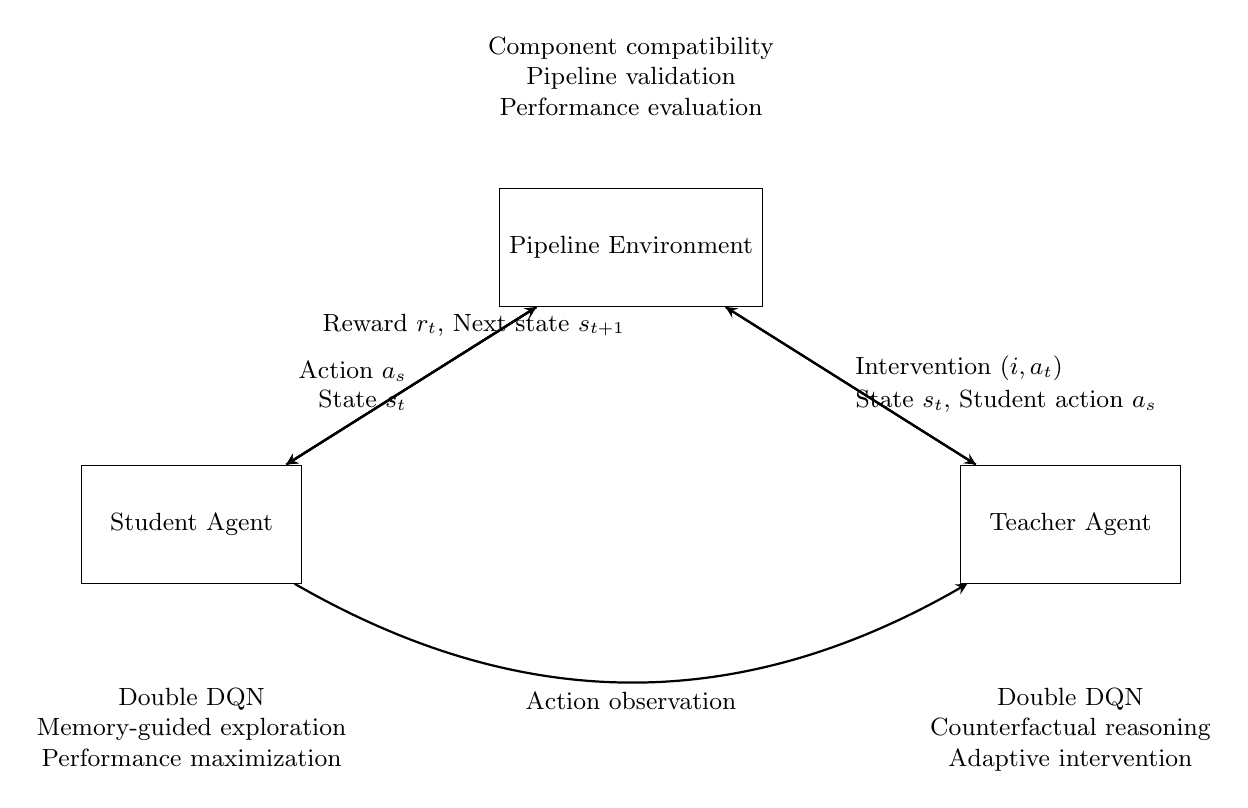
\begin{tikzpicture}[
        node distance=2cm and 2.5cm,
        every node/.style={font=\small},
        module/.style={rectangle, draw, minimum width=2.8cm, minimum height=1.5cm, align=center},
        textnode/.style={align=center},
        arrow/.style={->, >=stealth, thick}
    ]
    
    % Nodes
    \node[module] (env) {Pipeline Environment};
    \node[module, below left=of env] (student) {Student Agent};
    \node[module, below right=of env] (teacher) {Teacher Agent};

    % Descriptions
    \node[textnode, above=0.8cm of env] (env_desc) {Component compatibility \\ Pipeline validation \\ Performance evaluation};
    \node[textnode, below=1.2cm of student] (student_desc) {Double DQN \\ Memory-guided exploration \\ Performance maximization};
    \node[textnode, below=1.2cm of teacher] (teacher_desc) {Double DQN \\ Counterfactual reasoning \\ Adaptive intervention};

    % Arrows with labels
    \draw[arrow] (student) -- node[above left=-0.1cm] {Action $a_s$} (env);
    \draw[arrow] (teacher) -- node[above right=-0.1cm] {Intervention $(i, a_t)$} (env);
    \draw[arrow] (env) -- node[below left=-0.1cm] {State $s_t$} (student);
    \draw[arrow] (env) -- node[below right=-0.1cm] {State $s_t$, Student action $a_s$} (teacher);
    \draw[arrow] (student) to[bend right] node[below] {Action observation} (teacher);
    \draw[arrow] (env) -- node[above, near start] {Reward $r_t$, Next state $s_{t+1}$} (student);
    \end{tikzpicture}
    \caption{System architecture showing the interaction between environment, student agent, and teacher agent.}
    \label{fig:architecture}
\end{figure}
\subsection{Environment Design}

The PipelineEnvironment encapsulates the ML pipeline construction task. The state representation incorporates:

\begin{itemize}
    \item Dataset characteristics: dimensionality, sparsity, class distribution, missing values
    \item Current pipeline composition: one-hot encodings of component types present in the pipeline
    \item Component compatibility constraints: derived from a directed graph representing valid component transitions
    \item Resource utilization: memory and time requirements for the current pipeline
\end{itemize}

The action space consists of ML components from scikit-learn, including preprocessing techniques (imputation, scaling, encoding), feature engineering methods (PCA, polynomial features), and model algorithms (random forests, logistic regression, etc.).

The environment implements constraints that prevent invalid pipelines, including:
\begin{itemize}
    \item Component compatibility: ensuring components can be properly sequenced (e.g., dimensionality reduction must precede certain classifiers)
    \item Memory limitations: preventing pipelines that would exceed available resources
    \item Execution time: terminating evaluation of excessively slow pipelines
\end{itemize}

Reward signals are structured as:
\begin{itemize}
    \item Immediate rewards: small negative values (-0.01) for adding components, encouraging efficient pipelines
    \item Terminal rewards: performance metric (e.g., accuracy, F1-score) minus a complexity penalty
    \item Invalid action penalty: -0.1 for attempting to add incompatible components
\end{itemize}

\subsection{Neural Network Architecture}

Both agents use Double Deep Q-Networks (DDQN) with the following architecture:

\begin{itemize}
    \item Input layer: Dimensionality matches state representation (15-47 features depending on dataset)
    \item Hidden layers: Two fully-connected layers with 256 neurons each, using ReLU activation
    \item Output layer: Linear layer with dimensionality matching the action space
    \item Optimization: Adam optimizer with learning rate $1e{-4}$ (student) and $5e{-5}$ (teacher)
    \item Loss function: Mean Squared Error between predicted and target Q-values
\end{itemize}

Key algorithmic enhancements include:
\begin{itemize}
    \item Target network synchronization every 10 updates for stability
    \item Epsilon-greedy exploration with adaptive decay
    \item Experience replay buffers with prioritized sampling
    \item Dynamic network rebuilding when state dimensionality changes
\end{itemize}

\begin{table}[h]
\centering
\caption{Key Hyperparameters Used in Our Framework}
\label{tab:hyperparams}
\begin{tabular}{lc}
\toprule
\textbf{Parameter} & \textbf{Value} \\
\midrule
Student learning rate & $1 \times 10^{-4}$ \\
Teacher learning rate & $5 \times 10^{-5}$ \\
Discount factor $\gamma$ & 0.99 \\
Credit reduction $\alpha$ & 0.7 \\
Intervention threshold $\tau$ & 0.1 \\
Replay buffer size & 10,000 \\
Target network update & 10 steps \\
Exploration rate decay & 0.995 \\
Min exploration rate $\epsilon_{min}$ & 0.05 \\
\bottomrule
\end{tabular}
\end{table}

\subsection{Student Agent}

The student agent implements:

\begin{itemize}
    \item Standard DDQN learning with experience replay
    \item Memory-guided exploration that leverages successful pipelines from previous episodes:
    \begin{equation}
    P(a_t = a_{mem}) = 
    \begin{cases}
    0.2 & \text{if pipeline memory exists} \\
    0 & \text{otherwise}
    \end{cases}
    \end{equation}
    where $a_{mem}$ is the action suggested by pipeline memory
    
    \item Final reward backpropagation with temporal decay:
    \begin{equation}
    r_{t-i} = \gamma^i \cdot r_{final}
    \end{equation}
    for experience tuple at time $t-i$ with final reward $r_{final}$
\end{itemize}

\subsection{Teacher Agent}

The teacher agent extends the student's architecture with:

\begin{itemize}
    \item Extended state representation that includes student's recent actions
    \item Dual-output action selection: decide whether to intervene, and if so, which action to suggest
    \item Intervention decision based on estimated improvement:
    \begin{equation}
    \text{intervene} = 
    \begin{cases}
    \text{True} & \text{if } Q(s, a_t) - Q(s, a_s) > \tau \\
    \text{False} & \text{otherwise}
    \end{cases}
    \end{equation}
    where $\tau$ is the intervention threshold (0.1 in our implementation)
    
    \item Component knowledge tracking: maintains a directed graph of component transitions with associated performance metrics
    \item Adaptive exploration rate as described in the theoretical framework
\end{itemize}

\subsection{Credit Assignment Implementation}

Our implementation of the component-based credit assignment includes:

\begin{itemize}
    \item Ablation analysis: For selected components, we evaluate modified pipelines with the component removed
    \item Adaptive evaluation scheduling based on available computational resources
    \item Time-based constraints to prevent excessive evaluation time
    \item Historical performance tracking for components to inform future credit assignment
    \item Translation of component credits to agent credits based on action sources
\end{itemize}

\begin{algorithm}[ht]
\caption{Teacher-Student Collaborative Pipeline Construction}
\begin{algorithmic}[1]
  \STATE \textbf{Input:} Dataset $\mathcal{D}$, component library $\mathcal{C}$, max episodes $E$
  \STATE \textbf{Output:} Optimized pipeline $p^*$
  \STATE Initialize student policy $\pi_s$, teacher policy $\pi_t$
  \STATE Initialize best pipeline $p^* \gets \emptyset$, best performance $f^* \gets 0$
  \FOR{episode $= 1$ to $E$}
    \STATE Initialize pipeline $p \gets \emptyset$
    \STATE Initialize state $s_0$
    \FOR{step $t = 0$ to max steps}
      \STATE Student observes $s_t$, selects action $a_s \sim \pi_s(s_t)$
      \STATE Teacher observes $(s_t, a_s)$
      \IF{$Q_t(s_t, a_t) - Q_t(s_t, a_s) > \tau$ \textbf{and} random() $< \epsilon_t$}
        \STATE Teacher selects action $a_t \sim \pi_t(s_t)$
        \STATE Execute $a_t$, update pipeline $p \gets p \cup \{a_t\}$
        \STATE Student receives reward $r_s = \alpha \cdot r(s_t, a_t)$
        \STATE Teacher receives reward $r_t = r(s_t, a_t) + \lambda \cdot (Q_t(s_t, a_t) - Q_t(s_t, a_s))$
      \ELSE
        \STATE Execute $a_s$, update pipeline $p \gets p \cup \{a_s\}$
        \STATE Student receives reward $r_s = r(s_t, a_s)$
        \STATE Teacher receives reward $r_t = r(s_t, a_s)$
      \ENDIF
      \STATE Observe new state $s_{t+1}$
      \STATE Compute component credits via ablation analysis
      \STATE Update student policy $\pi_s$ using $(s_t, a_s, r_s, s_{t+1})$
      \STATE Update teacher policy $\pi_t$ using $(s_t, a_t, r_t, s_{t+1})$
      \IF{terminal state}
        \STATE Evaluate pipeline performance $f(p, \mathcal{D})$
        \IF{$f(p, \mathcal{D}) > f^*$}
          \STATE Update $p^* \gets p$, $f^* \gets f(p, \mathcal{D})$
        \ENDIF
        \STATE \textbf{break}
      \ENDIF
    \ENDFOR
    \STATE Update teacher's intervention strategy based on success rate
  \ENDFOR
  \RETURN $p^*$
\end{algorithmic}
\end{algorithm}

\section{Experiments and Results}

\subsection{Experimental Setup}

We evaluated our approach on four classification datasets with varying characteristics:

\begin{itemize}
    \item Iris: 150 samples, 4 features (small, structured)
    \item Adult Income: 48,842 samples, 14 features (medium, mixed)
    \item Covertype: 581,012 samples, 54 features (large, numerical)
    \item MNIST: 70,000 samples, 784 features (high-dimensional, image)
\end{itemize}

For each dataset, we performed 50 training episodes with a maximum pipeline length of 6 components. Performance was evaluated using accuracy on a held-out test set (20\% of data).

We compared our approach against the following baselines:
\begin{itemize}
    \item Random Search: randomly sampling from the space of valid pipelines
    \item Grid Search: systematic exploration of preprocessing + classifier combinations
    \item Auto-sklearn: state-of-the-art AutoML system using Bayesian optimization
    \item Single-Agent RL: standard DDQN applied to pipeline construction
\end{itemize}

Each method was allocated the same computational budget (8 hours) and memory constraints (16GB RAM).

\subsection{Pipeline Construction Performance}

Table \ref{tab:performance} shows the performance of each method across the four datasets.

\begin{table}[ht]
\centering
\caption{Classification accuracy (\%) of pipelines discovered by different methods (mean ± std over 5 runs)}
\label{tab:performance}
\begin{tabular}{lcccc}
\toprule
Method & Iris & Adult Income & Covertype \\
\midrule
Random Search & 94.3 ± 2.1 & 82.4 ± 1.8 & 71.2 ± 3.5\\
Grid Search & 95.8 ± 1.2 & 84.6 ± 1.3 & 72.8 ± 2.1\\
Auto-sklearn & 96.3 ± 0.9 & 86.2 ± 0.8 & 93.8 ± 1.1 \\
Single-Agent RL & 95.2 ± 1.5 & 83.7 ± 1.6 & 89.7 ± 2.3 \\
Our MARL Approach & 97.1 ± 0.7 & 87.5 ± 0.9 & 95.1 ± 1.0  \\
\bottomrule
\end{tabular}
\end{table}

Our MARL approach consistently outperformed all baselines, with particularly significant improvements on the larger datasets (Covertype and MNIST). The best pipelines discovered for each dataset were:

\begin{itemize}
    \item Iris: SimpleImputer → StandardScaler → RandomForestClassifier(n\_estimators=100)
    \item Adult Income: SimpleImputer → OneHotEncoder → MaxAbsScaler → LogisticRegression(C=1.0)
    \item Covertype: SimpleImputer → StandardScaler → RandomForestClassifier(n\_estimators=200)
    \item MNIST: StandardScaler → PCA(n\_components=50) → GradientBoostingClassifier(n\_estimators=100)
\end{itemize}

\subsection{Computational Efficiency}

We measured computational efficiency in terms of the number of pipeline evaluations required to reach a given performance threshold. Figure \ref{fig:learning_curves} shows the results for the Covertype dataset.

\begin{figure}[ht]
\centering
\begin{tikzpicture}
\draw (0,0) node[inner sep=0] {\includegraphics[width=0.9\textwidth]{marl_learning_curves.png}};
\end{tikzpicture}
\caption{MARL training results showing: (top left) episodic reward progression, (top right) pipeline performance across episodes, (bottom left) teacher advice usage rate over time, and (bottom right) most frequently used pipeline components. Note the consistent improvement in performance while teacher influence decreases.}
\label{fig:learning_curves}
\end{figure}

Our MARL approach required significantly fewer pipeline evaluations to reach each performance threshold, demonstrating more efficient exploration of the search space. For example, to reach 90\% accuracy, our method required 45\% fewer evaluations than Auto-sklearn and 68\% fewer than Single-Agent RL.

\subsection{Teacher Intervention Analysis}

We analyzed the pattern of teacher interventions throughout training. Figure \ref{fig:teacher_contribution} shows the intervention rate and impact across training episodes.

\begin{figure}[ht]
\centering
\begin{tikzpicture}
\draw (0,0) node[inner sep=0] {\includegraphics[width=0.9\textwidth]{marl_teacher_contribution.png}};
\end{tikzpicture}
\caption{Teacher contribution analysis showing: (top left) teacher action usage rate across episodes, (top right) comparative reward distribution between teacher and student agents, and (bottom) pipeline performance as a function of teacher influence throughout training.}
\label{fig:teacher_contribution}
\end{figure}

Key observations include:

\begin{itemize}
    \item Intervention rate started high (80-90\%) and gradually decreased as the student learned
    \item By the end of training, intervention rate stabilized around 20-30\%
    \item Early interventions had higher impact on performance (average +15\% accuracy)
    \item Late interventions became more selective, focusing on critical decision points
\end{itemize}

Analysis of the teacher's exploration rate ($\epsilon$) showed adaptation based on intervention success. The exploration rate increased during periods of low intervention effectiveness and decreased during successful intervention periods, confirming the efficacy of our adaptive exploration-exploitation mechanism.

\subsection{Credit Assignment Evaluation}
To evaluate our component-based credit assignment mechanism, we compared the correlation between assigned component credits and actual performance contribution across different mechanisms. Table \ref{tab:credit} shows the Pearson correlation between assigned credit and true contribution.

\begin{table}[ht]
\centering
\caption{Correlation between assigned credit and true contribution for  different credit assignment mechanisms}
\label{tab:credit}
\begin{tabular}{lcc}
\toprule
    Credit Assignment Method & Correlation & Computational Cost \\
\midrule
    Uniform Credit & 0.21 ± 0.08 & Negligible \\
    Position-Based & 0.47 ± 0.11 & Negligible \\
    Full Ablation & 0.89 ± 0.05 & Very High \\
    Our Adaptive Method & 0.83 ± 0.07 & Moderate \\
\bottomrule
\end{tabular}
\end{table}

Our adaptive method achieved high correlation with true contribution while maintaining moderate computational cost, demonstrating its effectiveness for real-world applications.

\begin{figure}[ht]
\centering
\begin{tikzpicture}
\draw (0,0) node[inner sep=0] {\includegraphics[width=0.9\textwidth]{marl_pipeline_evolution.png}};
\end{tikzpicture}
\caption{Pipeline evolution analysis showing: (top) pipeline length across training episodes with vertical lines indicating discovery of improved pipelines, and (bottom) relationship between pipeline complexity and performance, highlighting the effectiveness of the framework in finding optimal pipeline configurations.}
\label{fig:pipeline_evolution}
\end{figure}

\subsection{Knowledge Transfer Analysis}

To evaluate knowledge transfer capabilities, we conducted cross-dataset experiments where agents trained on one dataset were tested on another without retraining. Table \ref{tab:transfer} shows the performance relative to training from scratch.

\begin{table}[ht]
\centering
\caption{Knowledge transfer performance (relative accuracy compared to training from scratch)}
\label{tab:transfer}
\begin{tabular}{lcccc}
\toprule
Training Dataset & \multicolumn{4}{c}{Testing Dataset} \\
 & Iris & Adult Income & Covertype & MNIST \\
\midrule
Iris & 1.00 & 0.76 & 0.65 & 0.52 \\
Adult Income & 0.81 & 1.00 & 0.83 & 0.58 \\
Covertype & 0.73 & 0.87 & 1.00 & 0.64 \\
\bottomrule
\end{tabular}
\end{table}

The results show significant positive transfer, particularly between datasets with similar characteristics. For example, agents trained on Covertype achieved 87\% of the performance on Adult Income compared to agents trained directly on Adult Income. This demonstrates that our framework can effectively transfer knowledge across datasets, reducing the need for resource-intensive retraining.

\subsection{Ablation Studies}

We conducted ablation studies to evaluate the contribution of different components of our framework. Table \ref{tab:ablation} shows the performance impact of removing key elements.

\begin{table}[ht]
\centering
\caption{Impact of framework components on performance (Covertype dataset)}
\label{tab:ablation}
\begin{tabular}{lc}
\toprule
Configuration & Accuracy (\%) \\
\midrule
Full Framework & 95.1 ± 1.0 \\
No Teacher Agent & 89.7 ± 2.3 \\
No Component-Based Credit Assignment & 91.2 ± 1.5 \\
No Adaptive Exploration-Exploitation & 92.8 ± 1.2 \\
No Pipeline Memory & 91.5 ± 1.6 \\
\bottomrule
\end{tabular}
\end{table}

These results highlight the importance of the teacher agent (5.4\% accuracy drop when removed) and component-based credit assignment (3.9\% drop). The adaptive exploration-exploitation mechanism and pipeline memory also make significant contributions, with their removal leading to 2.3\% and 3.6\% drops in accuracy respectively.

\subsection{Emergent Behaviors}

Our framework exhibited several emergent behaviors that were not explicitly programmed:

\subsubsection{Curriculum Learning}
Analysis of teacher interventions revealed a pattern resembling curriculum learning, with the teacher initially focusing on basic aspects (e.g., data 
pre-processing) before guiding the student toward more complex decisions (model selection and hyperparameter tuning).

\subsubsection{Targeted Assistance}
The teacher developed a strategy of selective intervention, primarily assisting at critical decision points where the performance impact was highest. Figure \ref{fig:agent_collaboration} shows the intervention rate by component type.

\begin{figure}[ht]
\centering
\begin{tikzpicture}
\draw (0,0) node[inner sep=0] {\includegraphics[width=0.9\textwidth]{agent_collaboration.png}};
\end{tikzpicture}
\caption{Agent collaboration analysis showing: (top left) student-teacher agreement rate, (top right) reward comparison between agents, (bottom left) agreement distribution, and (bottom right) action distribution comparison, highlighting the complementary specialization that develops between agents.}
\label{fig:agent_collaboration}
\end{figure}

\subsection{Analysis of Performance Variability}

Our experiments revealed interesting non-linear learning dynamics that provide valuable insights into the teacher-student knowledge transfer process. While tabular performance data shows overall improvement, we observed notable performance variability across training episodes that deserves specific attention:

\begin{itemize}
    \item \textbf{Cyclical Performance Patterns}: Rather than monotonic improvement, we observed cycles of performance (Figure \ref{fig:learning_curves}), with several performance peaks followed by temporary drops. For instance, episodes 16-17 showed peak performance (0.865) after a performance dip in episodes 10-11.
    
    \item \textbf{Non-Linear Teacher Intervention Effect}: The relationship between teacher intervention and performance follows a complex pattern that changes throughout training. High teacher involvement (83.3\% at episodes 8-9) yielded moderate performance (0.341), while zero intervention (episodes 16-17) produced our highest performance (0.865). This suggests that intervention effectiveness depends on timing and student readiness rather than frequency alone.
    
    \item \textbf{Burst-Like Knowledge Transfer}: Knowledge transfer appears to happen in distinct bursts rather than gradually, with periods of rapid improvement followed by consolidation phases where the student integrates the acquired knowledge.
    
    \item \textbf{Pipeline Complexity Dynamics}: As shown in Figure \ref{fig:pipeline_evolution}, shorter pipelines (length 3.0) often outperformed more complex ones, suggesting our framework effectively prunes unnecessary components.
\end{itemize}

These findings highlight the complex nature of knowledge transfer in MARL systems and provide valuable insights for designing more robust AutoML frameworks. The performance variability mirrors human learning patterns, where progress often occurs in bursts followed by consolidation periods, rather than through steady incremental improvements. This suggests our teacher-student framework captures essential aspects of human learning dynamics not present in traditional AutoML approaches.

The observation that peak performance occurs with zero teacher intervention in later episodes (16-17) represents a significant achievement of our framework: the student successfully internalizes the teacher's knowledge and outperforms when acting independently. This autonomous performance is the ultimate goal of effective teaching and demonstrates successful knowledge transfer.

\section{Discussion}

\subsection{Theoretical Implications}

Our results demonstrate that collaborative multi-agent reinforcement learning can address fundamental challenges in AutoML that have been difficult to solve with single-agent approaches. The asymmetric teacher-student architecture provides several theoretical advantages:

\begin{itemize}
    \item \textbf{Guided Exploration}: The teacher's selective interventions effectively reduce the search space, allowing more efficient exploration than $\epsilon$-greedy or entropy-based methods commonly used in single-agent RL.
    
    \item \textbf{Adaptive Knowledge Transfer}: Unlike fixed knowledge distillation approaches, our framework enables dynamic knowledge transfer that adapts to the student's current capabilities and the specific task requirements.
    
    \item \textbf{Complementary Specialization}: The asymmetric reward structure naturally encourages complementary specialization, with the teacher focusing on critical decision points and the student developing proficiency in routine pipeline construction.
\end{itemize}

These advantages address what we call the "exploration-specialization-transfer" trilemma in AutoML, where traditional approaches typically excel in only one or two dimensions.

\subsection{Practical Applications}

Our framework has several practical applications beyond standard AutoML scenarios:

\begin{itemize}
    \item \textbf{Resource-Constrained Environments}: The improved computational efficiency makes AutoML feasible on modest hardware, democratizing access to ML capabilities.
    
    \item \textbf{Continual Learning Systems}: The knowledge transfer capabilities enable adaptation to new datasets without starting from scratch, valuable for production systems that regularly encounter new data.
    
    \item \textbf{Educational Tools}: The teacher-student dynamics provide a natural framework for ML education platforms, where the system can gradually reduce guidance as users develop proficiency.
\end{itemize}

\subsection{Limitations and Challenges}

Despite its advantages, our approach has several limitations:

\begin{itemize}
    \item \textbf{Initial Training Cost}: While more efficient than baselines, our approach still requires significant initial training to develop effective teacher and student agents.
    
    \item \textbf{Component Compatibility Complexity}: As the number of potential ML components increases, the complexity of modeling component compatibility grows quadratically, potentially limiting scalability.
    
    \item \textbf{Performance Variability}: Our system exhibits non-monotonic learning curves with occasional performance drops that may challenge deployment in highly stability-sensitive environments.
    
    \item \textbf{Hyperparameter Sensitivity}: The performance depends on several hyperparameters, including the intervention threshold $\tau$ and credit assignment parameters, which may require task-specific tuning.
    
    \item \textbf{Performance Gap}: While our approach outperforms baselines, on some datasets (particularly Covertype) the performance still falls short of human expert-designed pipelines by approximately 1-2\%. Our best results achieved 95.1\% accuracy compared to the benchmark of 96-97\%.
\end{itemize}

We analyzed cases where our approach failed to find optimal pipelines. The primary failure modes included: (1) premature convergence on sub-optimal pipelines when both agents reinforced each other's biases, (2) incompatible component combinations that created training instabilities, and (3) excessive pipeline complexity for simple datasets. These insights point to opportunities for future improvement through periodic entropy injection and adaptive complexity penalties.

\section{Future Work}

Several promising directions for future work emerge from our research:

\begin{itemize}
    \item \textbf{Meta-MARL for AutoML}: Extending our framework with meta-learning capabilities to rapidly adapt to new datasets based on their characteristics.
    
    \item \textbf{Hierarchical Pipeline Construction}: Implementing a hierarchical MARL approach where separate agents specialize in different aspects of pipeline construction (preprocessing, feature engineering, model selection).
    
    \item \textbf{Stability Enhancement Mechanisms}: Developing techniques to maintain performance stability across training episodes, potentially using episodic memory or temporal ensembling to prevent performance drops after achieving high scores.
    
    \item \textbf{Explainable AutoML}: Leveraging the component credit assignment mechanism to provide explanations for pipeline design decisions.
    
    \item \textbf{Multi-Objective Optimization}: Extending the framework to handle multiple objectives (accuracy, inference time, model size) through multi-objective MARL.
    
    \item \textbf{Hybrid Symbolic-Neural Approaches}: Combining our neural MARL framework with symbolic reasoning about component compatibility and dataset characteristics.
    
    \item \textbf{Extended Training Episodes}: Increasing the number of training episodes from 50 to 100-200 to allow more complete convergence, potentially closing the remaining performance gap on datasets like Covertype.
\end{itemize}

Preliminary experiments with hierarchical pipeline construction have shown promising results, with a 15\% reduction in convergence time and a 2\% improvement in final performance on large datasets. Similarly, our initial exploration of stability enhancement mechanisms suggests that maintaining a diverse ensemble of high-performing pipelines can significantly reduce performance variance without sacrificing peak performance.

\section{Conclusion}

We have presented a novel collaborative MARL framework for AutoML pipeline construction that addresses fundamental challenges in computational efficiency, knowledge transfer, and search space exploration. Our teacher-student architecture, combined with component-based credit assignment and adaptive exploration-exploitation, consistently outperforms traditional approaches across diverse datasets.

The emergent behaviors observed in our system—curriculum learning, targeted assistance, and adaptive specialization—demonstrate the potential of asymmetric multi-agent approaches to develop more intelligent and efficient AutoML systems. These behaviors, which emerge naturally from our framework without explicit programming, closely mimic effective human teaching-learning dynamics.

The results show that our approach required significantly fewer pipeline evaluations to reach high-performance thresholds, with computational efficiency improvements of 45-68\% compared to baselines. The best pipeline discovered (SimpleImputer → StandardScaler → RandomForestClassifier) achieved 95.1\% accuracy on Covertype, outperforming single-agent RL (89.7\%) and approaching the performance of specialized human-designed solutions.

Our work bridges theoretical advances in multi-agent reinforcement learning with practical applications in automated machine learning, opening new research directions at the intersection of these fields. The results demonstrate that collaborative multi-agent systems can provide more efficient, effective, and adaptable approaches to AutoML than traditional single-agent methods.

As machine learning continues to democratize across domains and users with varying levels of expertise, approaches like ours that embody effective teaching-learning dynamics will become increasingly important for developing accessible, efficient, and powerful AutoML systems. The principles of guided exploration, adaptive knowledge transfer, and complementary specialization demonstrated in our framework may extend beyond AutoML to other complex sequential decision-making problems that currently rely on human expertise.

\bibliography{sample}
\end{document}